\documentclass[article,nojss]{jss}\usepackage[]{graphicx}\usepackage[]{color}
% maxwidth is the original width if it is less than linewidth
% otherwise use linewidth (to make sure the graphics do not exceed the margin)
\makeatletter
\def\maxwidth{ %
  \ifdim\Gin@nat@width>\linewidth
    \linewidth
  \else
    \Gin@nat@width
  \fi
}
\makeatother


\usepackage{alltt}






\usepackage{float}
%\usepackage{framed}
\usepackage{subcaption}
\renewcommand{\subfloat}[2][need a sub-caption]{ \subcaptionbox{#1}{#2} }
\usepackage{amsmath}
\usepackage[ruled,vlined]{algorithm2e}
\usepackage{listings}
\usepackage[shortcuts]{extdash}
\usepackage{booktabs}
\usepackage{enumitem}


%\addbibresource{paper2.bib}
\def\cov{{\text{COV}}}
\def\E{{\text{E}}}
\def\var{{\text{var}}}
\def\T{{\footnotesize{^{_{\sf T}}}}}
\setkeys{Gin}{width=0.45\textwidth}
\setcitestyle{square}




\newcommand{\class}[1]{`\code{#1}'}
\newcommand{\fct}[1]{\code{#1()}}








\author{Ruoyong Xu\\University of Toronto
   \And Patrick Brown\\University of Toronto
   \And Pierre L’Ecuyer\\University of Montr\'eal}
\Plainauthor{Ruoyong Xu, Patrick Brown, Pierre L’Ecuyer}


\title{A tool set for random number generation on GPUs in R}
\Plaintitle{}
\Shorttitle{}


\Abstract{
We introduce the \proglang{R} package \pkg{clrng} which leverages the \pkg{gpuR} package and is able to generate random numbers in parallel on a Graphics Processing Unit (GPU) with the \pkg{clRNG} (OpenCL) library.  Parallel processing with GPU's can speed up computationally intensive tasks, which when combined with \proglang{R}, it can largely improve \proglang{R}’s downsides in terms of slow speed, memory usage and computation mode.  
%There is currently no \proglang{R} package that does random number generation on GPU, while random number generation is critical in simulation-based statistical inference and modeling. 
\pkg{clrng} enables reproducible research by setting random initial seeds for streams on GPU and CPU, and can thus accelerate several types of statistical simulation and modelling. 
The random number generator in \pkg{clrng} guarantees independent parallel samples even when \proglang{R} is used interactively in an ad-hoc manner, with sessions being interrupted and restored. This package is portable and flexible, developers can use its random number generation kernel for various other purposes and applications.  
}





\Keywords{GPU, \pkg{clrng} package, parallel computing, \pkg{clRNG} library}
\Plainkeywords{GPU, clrng package, parallel computing, clRNG library}


\Address{
  Ruoyong Xu, Patrick Brown\\
  Department of Statistics\\
  University of Toronto\\
  700 University Ave., Toronto, ON M5G 1Z5, Canada\\
  E-mail: \email{ruoyong.xu@mail.utoronto.ca}, \email{patrick.brown@utoronto.ca}\\\\ 
  Pierre L’Ecuyer\\
  Department of Computer Science and Operations Research\\
  University of Montr\'eal\\
  Pavillon André-Aisenstadt, 
   2920 chemin de la Tour, 
   Montréal, QC,  Canada,  H3T 1J4\\
  E-mail: \email{lecuyer@iro.umontreal.ca}}
\IfFileExists{upquote.sty}{\usepackage{upquote}}{}
\begin{document}
%\SweaveOpts{concordance=TRUE}



\section[Introduction]{Introduction}

% Why?
% 
% gpu massively parallel and relatively cheap, useful for stats
% there are gpu packages in R, gpuR
% no random numbers yet.  complicated to do on gpu, need multiple seeds becuase of parallel generation
% reproducability: need to save current state and restore

In recent years, parallel computing with \proglang{R} \citep{r2021} has become a very important topic and attracted lots of interest from researchers \citep[see][for a review]{eddelbuettel2021parallel}. Although \proglang{R} is one of the most popular statistical software with many advantages, it has drawbacks in memory usage and computation mode aspects \citep{zhao_2016}. To be more specific, (1) \proglang{R} requires all data to be loaded into the main memory (RAM) and thus can handle a very limited size of data; (2) \proglang{R} is a single-threaded program, it can not effectively use all the computing cores of multi-core processors. Parallel computing is the solution to these drawbacks, for an overview of current parallel computing approaches with \proglang{R}, see CRAN Task View by \citet{cran2021} at \url{https://cran.r-project.org/web/views/HighPerformanceComputing.html}. 

Graphics Processing Units (GPUs) have the potential to make an important contribution to parallel computing with \proglang{R}. GPUs can perform thousands of computations simultaneously, which makes them powerful for doing massively parallel computing, and they are relatively cheap compared to multicore CPU's. Although there have been a number of \proglang{R} packages developed which provide some GPU capability, they inevitably come with some limitations. Packages such as \pkg{gputools}, \pkg{gpumatrix}, \pkg{cudaBayesreg}, \pkg{rpud} (available on github), are no longer maintained, the popular \pkg{tensorflow} \citep{tensorflow1} package uses GPU via \proglang{Python}, which makes it difficult to include as a dependency for new \proglang{R} packages. All of these mentioned packages are restricted to \proglang{R} users with NVIDIA GPUs. \pkg{gpuR} \citep{gpur1} is the only \proglang{R} package with a convenient and flexible interface between \proglang{R} and GPUs, and it is compatible with many GPU devices. By utilizing the \pkg{ViennaCL} \citep*{rupp2016viennacl} library, it provides a bridge between \proglang{R} and non-proprietary GPUs through the \proglang{OpenCL} (Open Computing Language) backend, which when combined with \pkg{Rcpp} \citep{rcpp1} gives a building block for other \proglang{R} packages. 

Random number generation is critical in simulation-based statistical inference, machine learning and many other scientific fields. While most random number generators are sequential, the \proglang{R} packages \pkg{parallel}, \pkg{future} \citep*{future1.19.1} and \pkg{rlecuyer} \citep{sevcikova2015package} are able to generate random numbers in parallel on multicore CPUs. More specifically, \pkg{parallel} writes an interface for the \pkg{RngStreams}, a \proglang{\texttt{C++}} library by \cite{l2002object} which is based on a combined multiple-recursive generator (MRG) MRG32k3a. \pkg{future} and \pkg{rlecuyer} also uses the combined MRG algorithm for generating random numbers. For up-to-date review papers on the generation of random numbers on parallel devices, and GPUs in particular, see:  \cite{rLEC15a,rLEC17p,rLEC21a}.


The \pkg{clrng} package described here is currently the only \proglang{R} package that provides facilities for generating random numbers in parallel on GPU. Accomplishing this is complicated because each process must produce an independent (non-overlapping) sequence of random numbers, and in order to ensure reproducibility it should be possible to save and restore the current state of each stream of random numbers at any point.  By leveraging the \pkg{gpuR} package, \pkg{clrng} provides an extensible framework for \proglang{R} package developers to make use of these facilities in \proglang{C} or \proglang{OpenCL} code, and the random number generators guarantee independent parallel samples even when \proglang{R} is used interactively in an ad-hoc manner, with sessions being interrupted and restored.
%and can generate random numbers on GPU by using the \proglang{clRNG} \citep{l2015clrng} library in \proglang{OpenCL}, and can thus accelerate several types of statistical simulation and modelling.


The remaining sections are organized as follows:
In Section 2, we introduce streams and the use of streams in work-items on a GPU device for generating uniform random numbers, and the usage of \fct{runifGpu}.
In Section 3, we introduce two non-uniform RNGs in \pkg{clrng}, as examples for users to develop other RNGs of interest on GPUs in \proglang{R}.
In Section 4, we apply GPU-generated uniform random numbers in Monte Carlo simulation for Fisher’s exact test, we introduce how the random numbers are used and how the algorithm is parallelized and implemented on GPU. Then we provide two real data examples to demonstrate the function usage and its \proglang{R} performance.
In Section 5, we show a useful application of normal random numbers on GPU, using them to simulate batches of Gaussian random surfaces with Mat\'ern covariance matrices simultaneously, the simulation also uses GPU-enabled functions from our other package \pkg{gpuBatchMatrix}.
Finally, the paper concludes with a short summary and a discussion in Section 6.






\section{Uniform random number generation} \label{}
Uniform random number generators (RNGs) are the foundation for simulating random numbers from all types of probability distributions. \cite{l2012random} summarized the usual two steps to generate a random variable in computational statistics: (1) generating independent and identically distributed (i.i.d.) uniform random variables on the interval $(0, 1)$, (2) applying transformations to these i.i.d. $U(0, 1)$ random variables to get samples from the desired distribution. \cite{l2012random} and \cite{robert2004random} present many general transformation methods for generating non-uniform random variables, for example, the most frequently used inverse transform method, the Box-Muller algorithm \citep{box1958note} for Gaussian random variable generation, and so on, which are all built on uniform random variables. %In the rest paper, ``RNG'' refers to uniform pseudo random number generator.


\proglang{clRNG} \citep{l2015clrng} is an \proglang{OpenCL} library for uniform random number generation, it provides four different RNGs: the MRG31k3p, MRG32k3a, LFSR113, and Philox-4×32-10 generators. These four RNGs use different types of constructions. The \pkg{clrng} package uses the MRG31k3p RNG, making it able to generate random numbers on GPUs. We choose MRG31k3p as the base generator for the following reasons:  the original \pkg{RNGStreams} package \citep{l2002object} was built with MRG32k3a, which was designed to be implemented in double precision, and not with 32-bit integers. The MRG31k3p generator was designed later, specifically for 32-bit integer arithmetic, so it runs faster on the 32-bit GPUs. It is also faster than Philox-4×32-10. The MRG31k3p generator was introduced by \cite{rLEC00b}. MRG31k3p was also statistically tested extensively and successfully, \cite[see][]{rLEC07b}.    




In what follows, we will illustrate how to create streams and how to use streams to generate uniform random numbers. 

%THE PROBLEM:  each process needs to be independent, there's a risk of overlap.  solution: streams.  mrg31kp3 a stream is a vector of three positive integers.  initial state is first stream, compute new streams sequentially.
\subsection{Creating streams}\label{createstreams}
When a RNG is called in parallel processes or successively called at several places in a program in \proglang{R}, random number generation would be more complicated because there is no guarantee that the streams (analogous to \code{.Random.seed} in \proglang{R}) do not overlap, and thus the generated sequences of random numbers may have dependence. \pkg{clrng} uses multiple distinct streams that are used in work-items that executes in parallel on a GPU device. A popular way of obtaining multiple streams is to take an RNG with a long period and cut the RNG's sequence into very long disjoint pieces of equal length $Z$, and use each piece as a separate stream. Creating a new stream amounts to computing its starting point. Each of these streams can also be partitioned into substreams with equally-spaced starting points \citep{l2002object, rLEC15a}, although this is not currently implemented in \pkg{clrng}. In general, a stream object contains three elements: the current state of the stream, the initial state of the stream (or seed). Streams are created sequentially in the way that whenever the user creates a new stream, the software automatically jumps ahead by $Z$ steps to find its initial state, and the three states in the stream object are set to it. 


In the \proglang{clRNG} library, the MRG31k3p RNG's entire period of length approximately $2^{185}$ is divided into approximately $2^{51}$ non-overlapping streams of length $Z = 2^{134}$. %Each stream can be further partitioned into substreams of length $2^{72}$. 
The state (and seed) of each stream is a vector of six 31-bit integers. This size of state is appropriate for having streams running in work-items on GPU cards, while providing a sufficient period length for most applications. The initial state of the first stream (also called ``initial seed of the package'' or ``initial seed of the stream creator'' in \proglang{clRNG}) for the MRG31k3p RNG is by default $(12345, 12345, 12345, 12345, 12345, 12345)$. 


%The function \fct{clrngMrg31k3pCreateStreams} from \proglang{clRNG} creates streams on the host using the MRG31k3p RNG. If we want to use the streams in work-items on a GPU device, the streams have to be copied from the host to the global memory of the GPU device, and then each work-item copies the current states only of the streams to its private memory. 
\fct{setBaseCreator} sets the initial state of the first stream that is created, it plays a role in \pkg{clrng} like the function \fct{SetPackageSeed} in \pkg{RngStreams} and \fct{clrngSetBaseCreatorState} in \pkg{clRNG}. \pkg{clrng} is able to create streams both on the host and on the GPU device. The \fct{createStreamsCpu} function does the former. The \proglang{R} output below creates 4 streams on the host. 
%is an interface function of \fct{clrngMrg31k3pCreateStreams} that creates streams on host as \proglang{R} matrices, see the \proglang{R} output below, where we created 4 streams on the host using \fct{createStreamsCpu}, after transposing \code{myStreamsCpu}, each column of the matrix is a stream, creating streams on host makes it easy for us to view and check the streams behavior. Substreams are not created in \pkg{clrng} because currently we use one stream per work-item. 
\begin{CodeChunk}
\begin{CodeInput}
R> # creating streams on CPU
R> library("clrng")
R> setBaseCreator(rep(12345, 6))
R> myStreamsCpu <- createStreamsCpu(4)
R> t(myStreamsCpu)
\end{CodeInput}
\begin{CodeOutput}
##        [,1]       [,2]       [,3]       [,4]
##  [1,] 12345  336690377  502033783  739421137
##  [2,] 12345  597094797 1322587635 1475938232
##  [3,] 12345 1245771585 1964121530  730262207
##  [4,] 12345   85196284 1949818481 1630192198
##  [5,] 12345  523477687 1607232546  324551134
##  [6,] 12345 2094976052 1462898381  795289868
##  [7,] 12345  336690377  502033783  739421137
##  [8,] 12345  597094797 1322587635 1475938232
##  [9,] 12345 1245771585 1964121530  730262207
## [10,] 12345   85196284 1949818481 1630192198
## [11,] 12345  523477687 1607232546  324551134
## [12,] 12345 2094976052 1462898381  795289868
\end{CodeOutput} 
\end{CodeChunk} 

\fct{setBaseCreator} has a single argument, the state of the first stream which defaults to a vector of 12345's.  
The argument of \fct{createStreamsCpu} is the number of streams to create.  Normally users would create many more than the four presented here, as most GPU's have thousands of work items.  The default number of streams is 1024.


We move streams to the GPU by converting them to a `\code{vclMatrix}'.
\begin{CodeChunk}
\begin{CodeInput}
R> myStreamsGpu = vclMatrix(myStreamsCpu)
\end{CodeInput} 
\end{CodeChunk} 

Equivalently, \fct{createStreamsGpu} creates streams directly on the GPU and returns a `\code{vclMatrix}', which makes it slightly more efficient when the number of streams is large.  

There are a few important notes on the usage of these above functions.
\begin{itemize}
\item Calling \fct{setBaseCreator} creates a hidden object \code{.Random.seed.clrng}, which (unlike the standard \code{.Random.seed}) controls the creation of new streams (not random numbers).   We allow users to call \fct{setBaseCreator}  at any time. \fct{setBaseCreator} should be called once before \fct{createStreamsCpu} and \fct{createStreamsGpu} if they would like to select their own initial seeds, or never, in which case streams take the package's default initial seed.  Otherwise, there is a small probability of producing streams which overlap.
\item Users may switch between \fct{createStreamsCpu} and \fct{createStreamsGpu} in the same program, calling either will read and update \code{.Random.seed.clrng}.  This is not recommended as it causes unnecessary data transfer between host and device.
\item If an \proglang{R} session is restarted during a task, as long as users saved the \proglang{R} environment (which Rstudio does automatically), the initial states (seeds) of the newly created streams will carry on from the last streams' seed from the previous \proglang{R} session.
\item Objects on the GPU are lost when an R session is restarted, even if the workspace is saved.  The object \code{myStreamsGpu} will remain in the workspace if the session is restarted, but the GPU memory containing \code{myStreamsGpu}'s data will no longer be accessible and an error will occur if the object is accessed.  To retain streams when a session is restarted the streams should be copied to the CPU with \code{as.matrix}.
\end{itemize}

Unlike \proglang{R}'s standard random number generators, the streams need to be explicitly specified when generating random numbers with \code{clrng}.  It would be possible to hide streams from the user by storing them as a hidden object, which the \pkg{rlecuyer} package does to some extent, we have chosen not to do so for two reasons.  First, the streams would need to be stored on the CPU and transferred to and from the GPU every time they were used.
Second, computations might be distributed across multiple GPU devices or multiple computers, and being explicit about which streams are used where ensures reproducibility and avoids the possibility that the same streams might be used on different devices without the user being aware.







\subsection{Generating uniform random numbers}

The streams created sequentially are used by work-items (the GPU analogy of CPU cores) on a GPU to generate random numbers. In \pkg{clrng} each work-item takes one distinct stream to generate random numbers, so the number of streams created should always equal (or exceed) the maximum number of work items likely to be used. The main part of the kernel (functions for execution on the GPU) for generating uniform random numbers is shown in Listing \ref{lst:uniformkernel}. Kernels are written in the \proglang{C}-like \proglang{OpenCL} language, in which \code{__kernel} declares a function as a kernel, and the \code{__global} prefix to the pointer kernel arguments specifies that they point to global memory space accessible to all work items.  Users can set the argument \code{verbose=2} in the random number generator to print out the kernel, which is slightly more complex than the code in Listing \ref{lst:uniformkernel}. 
  
Here the pointers \code{streams} and \code{out} refer to the streams and the  output matrix respectively, which are stored in global memory. \code{Nrow} and \code{Ncol} represent row and column number of the matrix \code{out} respectively.   \code{Npad} is the "internal" number of columns, and \code{out} is an \code{Nrow} by \code{Ncol} submatrix of a larger \code{Nrow} by \code{Npad} matrix.

Each stream's current state is copied to the private memory of each work-item by the function \fct{streamsToPrivate}, in which \code{g1} and \code{g2} point to the first three and second three elements of stream states.
The object \code{startvalue} gives the position of the work item's stream in the \code{streams} object and is computed with the
\code{NpadStreams} object defined in a macro not shown here.   

The function \fct{clrngMrg31k3pNextState} generates an uniform random integer between 1 and 2147483647,  and then scaled to be in the interval $(0,1)$ by multiplying it by a constant \code{mrg31k3p\_NORM\_cl} (defined to be $1/2147483648$). If to generate random integers, \code{temp} is not scaled. At the end of generating random numbers, streams are transferred back to global memory through the function \fct{streamsFromPrivate}.

\begin{lstlisting}[language=C,basicstyle=\small,label={lst:uniformkernel},caption= Uniform random numbers generation kernel.]
__kernel void mrg31k3pMatrix(
  __global int* streams,
  __global float* out,
  int Nrow, int Ncol, int Npad){

int Drow, Dcol;
uint g1[3], g2[3];
double temp;
const int startvalue = (get_global_id(0) + 
get_global_size(0) * get_global_id(1)) * NpadStreams;

streamsToPrivate(streams,g1,g2,startvalue);

for(Drow = get_global_id(0); Drow < Nrow;
    Drow += get_global_size(0)){

    for(Dcol = get_global_id(1); Dcol < Ncol; 
        Dcol += get_global_size(1)){

        temp = fact * clrngMrg31k3pNextState(g1, g2);
        out[Drow * Npad + Dcol] = temp;

  }//Dcol
}//Drow

streamsFromPrivate(streams,g1,g2,startvalue);

}//kernel
\end{lstlisting}

%Figure \ref{fig:1} illustrates how this kernel executes in practice with a simple example. Suppose we have a $2 \times 4$ NDRange ((a) in Figure \ref{fig:1}) and want to create a $4 \times 6$ matrix ((b) in Figure \ref{fig:1}) of uniform random numbers. In each grid of (a) that represents a work-item, there are two rows of numbers, the number in the above row is the stream index (from 0 to 7), and a pair of numbers in the second row is the 2-dimensional global ID of the work-item. Each stream object is passed to each work-item. The number in a cell of the matrix corresponds to the stream index, it indicates which stream generates a random number for this matrix cell. %For example, stream 0 which is allocated in work-item $(0,0)$ generates a random number in matrix $(0,0)$ in the first iteration, then moves on to matrix $(0,2)$ and generates a random number there in the second iteration, in the third iteration it generates a random number in matrix $(0,4)$ and so on until it goes out of the matrix range in the next iteration.
% \begin{figure}[ht]
%     \centering
%     \subfloat[]{{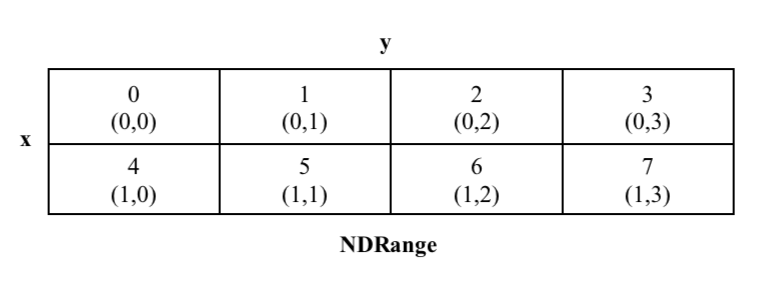
\includegraphics[width=8cm]{/home/ruoyong/diseasemapping/pkg/gpuRandom/inst/documents/paper1_2021_5/f1} }}
%     \qquad
%     \subfloat[]{{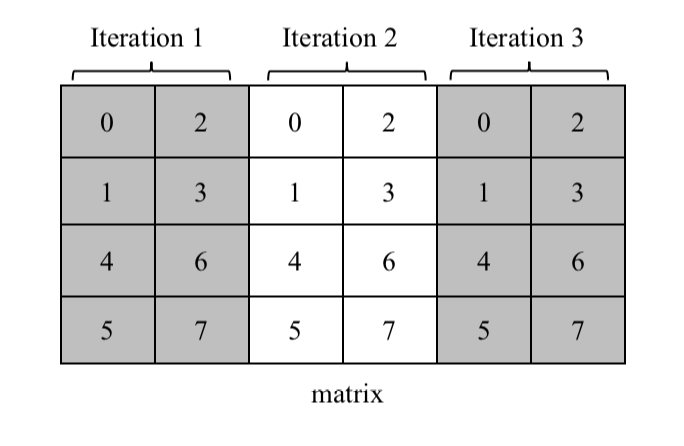
\includegraphics[width=8cm]{/home/ruoyong/diseasemapping/pkg/gpuRandom/inst/documents/paper1_2021_5/f2} }}
%     \caption{Using streams to produce a $4 \times 6$ matrix of random U(0,1) numbers. \label{fig:1}}
% \end{figure}

Now we use the 4 streams created in section \ref{createstreams} to generate a vector of double-precision i.i.d. $U(0,1)$ random numbers with \fct{runifGpu}. To view the generated random numbers, we need to convert them to \proglang{R} vectors or matrices, by doing this, the random numbers are moved from the global memory of the GPU device to the host.
\begin{CodeChunk}
\begin{CodeInput}
R> sim_1 = runifGpu(n = 8, streams = myStreamsGpu, Nglobal = c(2,
+    2))
R> as.vector(sim_1)
\end{CodeInput}
\begin{CodeOutput}
## [1] 0.735 0.842 0.614 0.216 0.110 0.870 0.649 0.170
\end{CodeOutput} 
\end{CodeChunk} 

The arguments of the \fct{runifGpu} are described as follows:
\begin{itemize}
\itemsep0em 
  \item \code{n}: Either a scalar giving the number of samples to generate or a vector of length 2 specifying the size of a matrix to be output.
  \item \code{streams}: Streams for random number generation, which must be stored on the GPU as a \code{vclMatrix} object.
  \item \code{Nglobal}: Number of work items, by default it is set as $(64,8)$.
  \item \code{type}: \code{double}, \code{float} or \code{integer}, the format of generated random numbers, defaults to \code{double}.
  \item \code{verbose}: Print extra information if $\text{verbose} > 1$.
\end{itemize}

The object returned is either a \code{vclMatrix} or \code{vclVector}, depending on whether \code{n} is two- or one-dimensional.  Reusing \code{myStreamsGpu} will produce a vector different form \code{sim_1}, as the current states of the streams in \code{myStreamsGpu} have advanced by two positions (each of the 4 work item generated 2 random numbers).  

As mentioned earlier, streams on the GPU do not remain in the memory when an \proglang{R} session is restarted. There are two ways to reproduce results, depending on how the program calls streams creator.
The simpler way to reproduce is just to have a single program in an \proglang{R} script file with the initial seed for the creator set at the beginning.  But it is important that the program always creates the streams in exactly the same order, for example, like the toy \proglang{R} program for demonstration below, we can reproduce the random matrix \code{sim_mat} just by keeping a record of the initial seed \code{c(11,22,33,44,55,66)}.
\begin{CodeChunk}
\begin{CodeInput}
R> library("clrng")
R> setBaseCreator(c(11, 22, 33, 44, 55, 66))
R> sim_mat <- matrix(0, nrow = 10, ncol = 6)
R> for (i in 1:10) {
+    if (i%%2 == 0) {
+        streams1 <- createStreamsGpu(4)
+        sim_mat[i, ] <- as.vector(clrng::rnormGpu(n = 6, streams = streams1,
+            Nglobal = c(2, 2)))
+    } else if (i == 3) {
+        streams2 <- createStreamsGpu(4)
+        sim_mat[i, ] <- as.vector(runifGpu(n = 6, streams = streams2,
+            Nglobal = c(2, 2)))
+    } else {
+        streams3 <- createStreamsGpu(8)
+        sim_mat[i, ] <- as.vector(rexpGpu(n = 6, streams = streams3,
+            Nglobal = c(4, 2)))
+    }
+}
R> sim_mat
\end{CodeInput} 
\end{CodeChunk} 


Were we to replace the \code{for} loop above with a parallel equivalent (i.e.\ \code{mcmapply}), the order of stream creation could change with each program execution and the result would not be reproducible.  For more complicated applications, we recommend users to save the matrix of streams (current states and initial states) on the CPU in a file as a \code{.rds} object. And later recall the saved streams for regenerating results, the streams will start from their current states after they are loaded. This is a safer way than the previous one for reproducing results in simulations. Below we show the code that saves streams to a data file called \code{myStreams.rds} on CPU and then load it back and transfer it to a `vclMatrix' \code{streams_saved} on GPU, and using it to (re)generate some Normal random numbers.
\begin{CodeChunk}
\begin{CodeInput}
R> saveRDS(as.matrix(myStreamsGpu), "myStreams.rds")
R> # Load the streams object as streams_saved
R> streams_saved <- vclMatrix(readRDS("myStreams.rds"))
R> clrng::rnormGpu(n = 6, streams = streams_saved, Nglobal = c(2,
+    2))
\end{CodeInput} 
\end{CodeChunk} 






\section{Some non-uniform random number generation}
\subsection{Normal random number generation}
We apply the Box-Muller transformation to $U(0,1)$ random numbers to generate standard normal random numbers. As shown in Algorithm \ref{algorithm1}, Box-Muller algorithm takes two independent, standard uniform random variables $U_1$ and $U_2$ and produces two independent, standard Gaussian random variables $X$ and $Y$, where $R$ and $\Theta$ are polar coordinate random variables. %The derivation basically uses transformation from Cartesian coordinates to polar coordinates to represent two independent, Normally distributed random variables. 
The Box-Muller algorithm is a very good choice for Gaussian transform on GPU's compared to other transform methods \citep{howes2007efficient}, because this algorithm has no branching or looping, which are the things GPU's are poor at. 

\begin{algorithm}[ht] 
\SetAlgoLined
 1, Generate $U_1$, $U_2$ i.i.d. from $U (0,1)$ \;
 2, Define \begin{align*} 
& R = \sqrt{-2*\log U_1},\\
&  \Theta = 2\pi*U_2,\\
&  X=R*\cos(\Theta),\\
& Y=R*\sin(\Theta);\;\end{align*}
 3, Take $X$ and $Y$ as two independent draws from $N(0,1)$\;
 \caption{Box-Muller algorithm.}
 \label{algorithm1}
\end{algorithm}


Listing \ref{lst:normal} shows a fragment of the kernel that generates standard Gaussian random numbers. The kernel has work items operating in pairs with shared local memory, the $U_1$ and $U_2$ are generated in parallel and stored in the two-dimenstional vector \code{part} below.  The \code{get_local_id(1)} command will return either zero or one, for the first and second item in the pair respectively.   As the work-items in a work-group proceed at different rates, \code{barrier(CLK_LOCAL_MEM_FENCE)} ensures correct ordering of memory operations to local memory, so that Gaussian random numbers $(X_1,Y_1), \dots, (X_n,Y_n)$ are generated in pairs correctly, errors such as $(X_n, Y_{(n-1)})$ or $(X_{(n-1)}, Y_{(n)})$ are avoided.



\begin{lstlisting}[language=C,basicstyle=\small,label={lst:normal},breaklines=true, escapeinside={(*@}{@*)}, caption = Normal random numbers generation kernel.]
__kernel void mrg31k3pMatrix(
  __global int* streams,
  __global double* out,
  int Nrow, int Ncol, int Npad, int NpadStreams){

int Drow, Dcol;
uint g1[3], g2[3];
int startvalue = (get_global_id(0) * get_global_size(1) + 
  get_global_id(1)) * NpadStreams;
const double fact[2] = { mrg31k3p_NORM_cl, TWOPI * mrg31k3p_NORM_cl };
const double addForSine[2] = { 0.0, - PI_2 };
local double part[2];

streamsToPrivate(streams,g1,g2, startvalue);

for(Drow=get_global_id(0); Drow < Nrow; Drow += get_global_size(0)){
  for(Dcol=get_global_id(1); Dcol < Ncol; Dcol += get_global_size(1)){
        
    part[get_local_id(1)] = fact[get_local_id(1)] * 
      clrngMrg31k3pNextState(g1, g2);
    barrier(CLK_LOCAL_MEM_FENCE);
    out[Drow * Npad + Dcol] = sqrt( -2.0*log(part[0]) ) * 
      cos(part[1] + addForSine[get_local_id(1)] );
    barrier(CLK_LOCAL_MEM_FENCE);
    
  }//Dcol
}//Drow
streamsFromPrivate(streams,g1,g2,startvalue);
}//kernel
\end{lstlisting}

%We illustrate in Figure \ref{fig3} how this kernel executes in practice with the previous toy example: to create a $4 \times 6$ matrix of Gaussian random numbers using a $2 \times 4$ NDRange. %Each stream is copied to the private memory of each work-item. 
%Work-items are organized to be in 1 by 2 work-groups as the random numbers are generated in pairs using the Box-Muller method. The shading on the grids in the NDRange distinguishes work-groups. The numbers in the third row in each gird of NDRange represents the local index of each work-item. Each work-group generates a pair of Gaussian random numbers \code{(X,Y)} in each iteration, where work-item of `\code{get_local_id(1)}$=0$' generates the \code{X} of a pair, and work-item of `\code{get_local_id(1)}$=1$' generates the \code{Y} of a pair. %Here with the loop iterating over columns, the cells of matrix are filled from left to right, that is, in the first iteration, the 8 work-items generate random numbers in the leftmost two columns (8 cells) of the matrix simultaneously, the second iteration fills random numbers in the middle two columns of the matrix, and the third iteration fills the rest two columns of the matrix simultaneously. %Therefore, each work-item generates one Gaussian random number in each iteration, The matrix filling process is the same as that shown in Figure \ref{fig:1}. 

% \begin{figure}[ht]%
%     \centering
%     \subfloat[]{{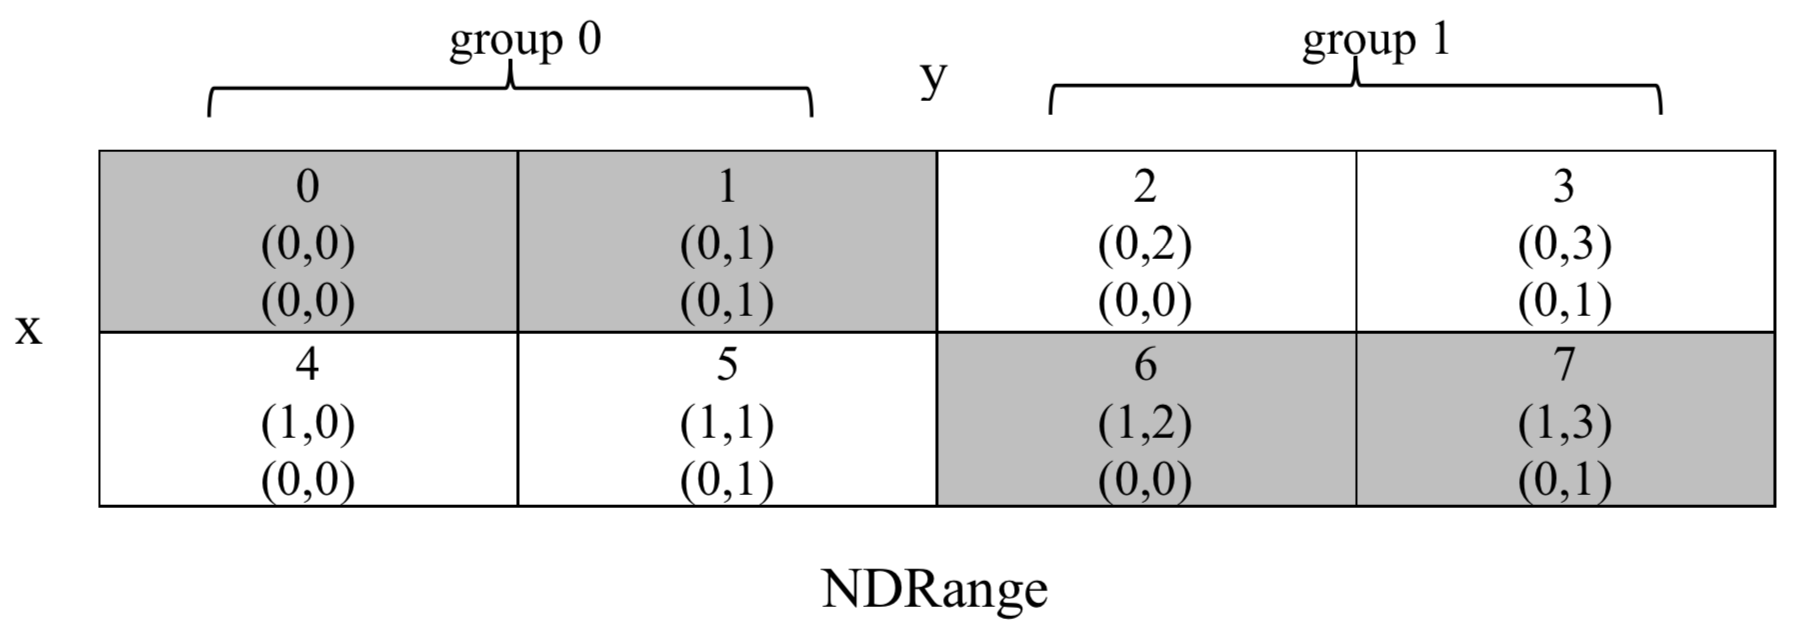
\includegraphics[width=8cm]{/home/ruoyong/diseasemapping/pkg/gpuRandom/inst/documents/paper1_2021_5/f3} }}%
%     \qquad
%     \subfloat[]{{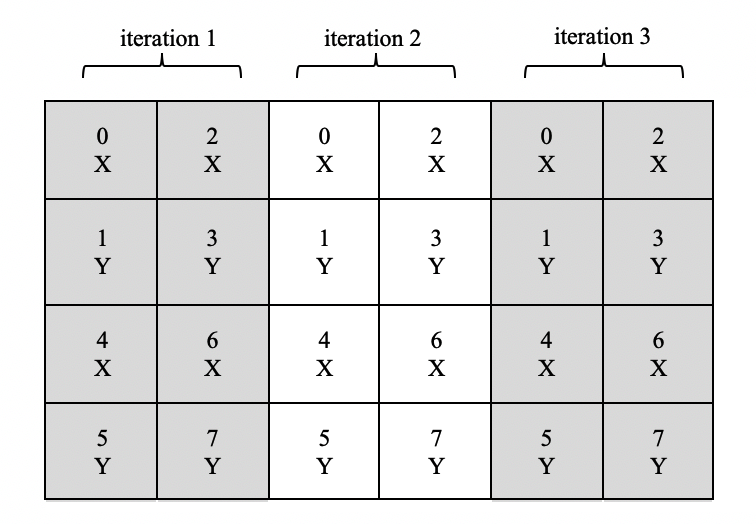
\includegraphics[width=8cm]{/home/ruoyong/diseasemapping/pkg/gpuRandom/inst/documents/paper1_2021_5/f4} }}%
%     \caption{Using streams to produce a $4 \times 6$ matrix of normal random numbers.}%
%     \label{fig3}
% \end{figure}
 

Below we generate a large-size matrix of 100 million double-precision Gaussian random numbers, and compare the run-time between using \fct{stats::rnorm} and \fct{rnormGpu}. The best performance we have seen using \fct{rnormGpu} is above 170 times faster with $512 \times 128$ work-items than using the standard (and single-threaded) \fct{stats::rnorm}. The difference in elapsed time becomes larger when matrix size increases.
\begin{CodeChunk}
\begin{CodeInput}
R> streams <- createStreamsGpu(512 * 128)
R> system.time(rnormGpu(c(10000, 10000), streams = streams, Nglobal = c(512,
+    128), type = "double"))
\end{CodeInput}
\begin{CodeOutput}
##    user  system elapsed 
##   0.052   0.003   0.055
\end{CodeOutput} 
\end{CodeChunk} 

\begin{CodeChunk}
\begin{CodeInput}
R> system.time(matrix(rnorm(10000^2), 10000, 10000))
\end{CodeInput}
\begin{CodeOutput}
##    user  system elapsed 
##   6.686   0.799   7.478
\end{CodeOutput} 
\end{CodeChunk} 



\subsection{Exponential random number generation}
The exponential random variates are produced by applying the inverse transform method on i.i.d. $U(0,1)$ random numbers. The random variable $X \sim \text{Exponential}(\lambda)$ has cumulative distribution function $F_{X}(x)=1-e^{-\lambda x}$ for $x \geq 0$ and $\lambda > 0$. The inverse of $F_{X}(\cdot)$ is $F^{-1}_{X}(y)= -(1/ \lambda) \log (1-y)$, for $ 0 \leq y <1$. The kernel is not shown because it is mostly same as the kernel for uniform and normal random numbers, except for the part that does the inverse transform. %Developers can make use of our kernel for generating other types of random variables on GPU in \proglang{R}.

Below is an example that produces a $2 \times 4$ matrix of Exponential random numbers with expectation equal to 1.
\begin{CodeChunk}
\begin{CodeInput}
R> r_matrix <- rexpGpu(c(2, 4), rate = 1, myStreamsGpu, Nglobal = c(2,
+    2), type = "double")
R> as.matrix(r_matrix)
\end{CodeInput}
\begin{CodeOutput}
##      [,1]  [,2]  [,3]  [,4]
## [1,] 1.00 0.689 2.218 1.167
## [2,] 1.48 1.205 0.406 0.241
\end{CodeOutput} 
\end{CodeChunk} 

The arguments of the \fct{rexpGpu} are described as follows:
\begin{itemize}
\itemsep0em 
  \item \code{n}: A vector of length 2 specifying the row and column number if to create a matrix, or a number specifying the length if to create a vector.
  \item \code{streams}: Streams for random number generation, streams cannot be missing.
  \item \code{Nglobal}: Global index space. Default is $(64,8)$.
  \item \code{type}: ``double'' or ``float'' format of generated random numbers.
  \item \code{verbose}: Print extra information if $\text{verbose} > 1$. Default is set to 0.
\end{itemize}





\section{An application of uniform RNG: Fisher's simulation}
The GPU-generated random numbers can be applied in suitable statistical simulations to accelerate computations.
One application of GPU-generated random numbers in \pkg{clrng} is Monte Carlo simulation for Fisher's exact test. Fisher’s exact test is applied for analyzing usually $2 \times 2$ contingency tables when one of the expected values in table is less than 5. Different from methods which rely on approximation, Fisher's exact test computes directly the probability of obtaining each possible combination of the data for the same row and column totals (marginal totals) as the observed table, and get the exact p-value by adding together all the probabilities of tables as extreme or more extreme than the one observed. However, when the observed table gets large in terms of sample size and table dimensions, the number of combinations of cell frequencies with the same marginal totals gets very large, \cite[][p. 23]{mehta2011ibm} shows a $5 \times 6$ observed table that has 1.6 billion possible tables. Calculating the exact P-values may lead to very long run-time and can sometimes exceed the memory limits of your computer. Hence, the option \code{simulate.p.value = TRUE} in \fct{stats::fisher.test} is provided, which enables computing p-values by Monte Carlo simulation for tables larger than 2 $\times$ 2. 

The test statistic calculated for each random table is $-\sum_{i,j}\log(n_{ij}!), i=(1,\dots, I), j=(1,\dots,J)$, (i.e., minus log-factorial of table), where $I$ and $J$ are the row and column number of the observed table. This test statistic can also be independently calculated for a table by \fct{clrng::logfactSum}. Given an observed table and a number of replicates $B$, the Monte Carlo simulation for Fisher's exact test does the following steps: 
\begin{enumerate}
\setlength\itemsep{0em}
  \item Calculate the test statistic for the observed table.
    \item In each iteration, simulate a random table with the same dimensions and marginal totals as the observed table using the \fct{rcont2} algorithm, compute and optionally save the test statistic from the random table. 
    \item Count the number of iterations (\emph{Counts}) that have test statistics less or equal to the one from the observed table.
    \item Estimate p-value using $\frac{1 + \emph{Counts}}{B + 1}$.
\end{enumerate}

Step 1 and step 2-3 are done on a GPU with two kernels enqueued sequentially. For step 2, \fct{clrng::fisher.sim} adapted the function \fct{rcont2} used by \fct{stats::fisher.test} for constructing random two-way tables with given marginal totals. The algorithm \citep[see][]{patefield1981efficient} samples the entries row by row, one at a time, conditional on the values of the entries already sampled. The conditional probabilities for the possible values of the next entry are updated dynamically each time a new entry is sampled. Then this entry is sampled by standard inversion of the cumulative distribution function, using one $U(0,1)$ random number.  For an $I \times J$ table, this requires $(I-1)(J-1)$ random numbers (the last column and last row do not need to be sampled). Finally, one can compute the test statistic for this newly sampled table. On a GPU, this step can be replicated say $n$ times in parallel by creating $n$ distinct random streams and launching $n$ separate work-items. Each work-item takes a random stream as input, performs all of Step 2 and 3, and returns the value of the test statistic on the GPU. Computing the p-value on the CPU (Step 4) is then a trivial operation.  Step 2 of saving test statistics from the random tables is made optional, which can reduce the run-time. By the way, there are a lot of other more recent methods for sampling (larger) contingency tables, many of them use Markov Chain Monte Carlo, the use of streams and GPU would be quite different in that case. See for examples \citep{10.1214/13-AOS1131, KAYIBI2018298, dyer1997sampling}. Doing the \fct{fisher.sim} function on GPU opens up many possibilities for future work, the specific implementation we've done for the tables isn't necessarily the optimal one. 

The arguments of the \fct{clrng::fisher.sim} are described as follows:
\begin{itemize}
\setlength{\parskip}{0pt}
  \item \code{x}: A contingency table, a ``vclMatrix'' object.
  \item \code{N}: Number of simulation runs.
  \item \code{streams}: Streams for random number generation, streams cannot be missing.
  \item \code{type}: ``double'' or ``float'' of returned test statistics.
  \item \code{returnStatistics}: If TRUE, return all test statistics. 
  \item \code{Nglobal}: Global index space. Default is set as $(64,16)$.
\end{itemize}
Users request $N$ number of replicates, while the actual number of replicates to be executed on GPU is larger (\code{ceiling(N/prod(Nglobal))*prod(Nglobal)}). We show the advantage of \fct{clrng::fisher.sim} by computing the p-values for two real data examples: one with a relatively big p-value and another with a very small p-value, and compare the run-time with using \fct{stats::fisher.test} for each of the data sets on two computers: one with a very good CPU and an ordinary GPU, the other is equipped with an excellent GPU and an ordinary CPU. The \proglang{R} outputs for testing on computer 2 is shown in the following. 


 
\subsection{Comparing run-time: Monthly birth anomolies}\label{fisher_month}

The 2-way contingency table in Table \ref{tab:monthdata} comes from the 2018 Natality public use data from the Centers for Disease Control and Prevention’s National Center for Health Statistics \citep{National2018}.  The 2018 natality data file may be downloaded at \url{https://www.cdc.gov/nchs/data_access/VitalStatsOnline.htm}. Table \ref{tab:month} is a $12 \times 12$ table that shows frequencies for congenital anomalies of the newborn by birth month in 2018 within the United States. The column variables of these two tables represent the twelve categories of congenital anomalies of the newborn: 1) Anencephaly; 2) Meningomyelocele/Spina bifida; 3) Cyanotic congenital heart disease; 4) Congenital diaphragmatic hernia; 5) Omphalocele; 6) Gastrochisis; 7) Limb reduction defect; 8) Cleft lip with or without cleft palate; 9) Cleft palate alone; 10) Down syndrome; 11) Suspected chromosomal disorder; and 12) Hypospadias. 



\begin{table}

\caption{\label{tab:monthdata}Monthly counts of birth anomalies.\label{tab:month}}
\centering
\begin{tabular}[t]{lrrrrrrrrrrrr}
\toprule
  & Ane & Men & Cya & Her & Omp & Gas & Lim & Cle & Pal & Dow & Chr & Hyp\\
\midrule
Jan & 29 & 55 & 172 & 46 & 39 & 73 & 48 & 183 & 77 & 103 & 102 & 174\\
Feb & 25 & 45 & 175 & 35 & 31 & 55 & 34 & 142 & 81 & 115 & 100 & 180\\
Mar & 31 & 48 & 182 & 41 & 47 & 72 & 40 & 200 & 86 & 90 & 96 & 180\\
Apr & 34 & 45 & 186 & 36 & 32 & 75 & 42 & 173 & 56 & 87 & 90 & 193\\
May & 33 & 40 & 187 & 46 & 24 & 80 & 35 & 180 & 75 & 91 & 100 & 197\\
Jun & 34 & 48 & 189 & 35 & 33 & 75 & 45 & 154 & 74 & 102 & 100 & 182\\
Jul & 26 & 43 & 198 & 34 & 21 & 74 & 36 & 179 & 79 & 86 & 92 & 193\\
Aug & 24 & 41 & 189 & 44 & 43 & 62 & 48 & 183 & 88 & 109 & 94 & 194\\
Sept & 34 & 44 & 147 & 40 & 37 & 66 & 36 & 158 & 73 & 112 & 103 & 196\\
Oct & 25 & 43 & 207 & 45 & 31 & 65 & 49 & 181 & 77 & 108 & 115 & 220\\
Nov & 36 & 55 & 188 & 39 & 39 & 62 & 43 & 144 & 68 & 98 & 79 & 173\\
Dec & 23 & 48 & 196 & 31 & 31 & 71 & 31 & 177 & 86 & 86 & 73 & 156\\
\bottomrule
\end{tabular}
\end{table}





\begin{CodeChunk}
\begin{CodeInput}
R> # using GPU
R> streams <- createStreamsGpu(n = 256*64)
R> month_gpu <- vclMatrix(month, type = "integer")
R> system.time(result_month <- 
+  clrng::fisher.sim(month_gpu, 1e6, 
+     streams=streams, type="double", 
+     returnStatistics=TRUE,  Nglobal = c(256,64)))
\end{CodeInput}
\begin{CodeOutput}
##    user  system elapsed 
##   0.331   0.001   0.331
\end{CodeOutput} 
\end{CodeChunk} 

\begin{CodeChunk}
\begin{CodeInput}
R> unlist(result_month[c("threshold", "simNum", "counts")])
\end{CodeInput}
\begin{CodeOutput}
## threshold    simNum    counts 
##    -47955   1015808    409429
\end{CodeOutput}
\begin{CodeInput}
R> result_month$p.value
\end{CodeInput}
\begin{CodeOutput}
## [1] 0.403
\end{CodeOutput} 
\end{CodeChunk} 

We got 409429 cases whose test statistics are below the observed threshold based on an actual number of 1015808 simulations, so the p-value from \fct{clrng::fisher.sim} for this table is about $4.03\times 10^{-1}$, which is close enough to the p-value from \fct{stats::fisher.test}. \fct{clrng::fisher.sim} takes about 0.3 seconds, \pkg{clrng} accounts for 2.1\% of the elapsed time on CPU. 

 
\begin{CodeChunk}
\begin{CodeInput}
R> # using CPU
R> system.time(result_monthcpu <- stats::fisher.test(month, simulate.p.value = TRUE,
+    B = 1015808))
\end{CodeInput}
\begin{CodeOutput}
##    user  system elapsed 
##  15.019   0.016  15.024
\end{CodeOutput}
\begin{CodeInput}
R> result_monthcpu$p.value
\end{CodeInput}
\begin{CodeOutput}
## [1] 0.404
\end{CodeOutput} 
\end{CodeChunk} 




\subsection{Comparing run-time: Day-of-week birth anomolies}\label{fisher_week}

Table \ref{tab:week} is a $7 \times 12$ table shows frequencies for congenital anomalies of the newborn by birth day of week in 2018 within the United States. 

\begin{table}

\caption{\label{tab:weekdata}Day-of-week birth anomaly data\label{tab:week}}
\centering
\begin{tabular}[t]{lrrrrrrrrrrrr}
\toprule
  & Ane & Men & Cya & Her & Omp & Gas & Lim & Cle & Pal & Dow & Chr & Hyp\\
\midrule
Mon & 30 & 34 & 173 & 37 & 23 & 80 & 49 & 191 & 83 & 122 & 109 & 216\\
Tue & 60 & 121 & 383 & 80 & 83 & 131 & 71 & 349 & 146 & 164 & 168 & 352\\
Wed & 51 & 106 & 417 & 92 & 73 & 145 & 72 & 333 & 136 & 179 & 196 & 351\\
Thu & 60 & 86 & 362 & 69 & 74 & 120 & 85 & 326 & 132 & 220 & 187 & 359\\
Fri & 52 & 94 & 347 & 87 & 59 & 123 & 68 & 323 & 145 & 170 & 166 & 345\\
Sat & 52 & 63 & 323 & 67 & 64 & 135 & 73 & 316 & 170 & 189 & 188 & 357\\
Sun & 49 & 51 & 211 & 40 & 32 & 96 & 69 & 216 & 108 & 143 & 130 & 258\\
\bottomrule
\end{tabular}
\end{table}


\begin{CodeChunk}
\begin{CodeInput}
R> # using GPU
R> week_GPU <- gpuR::vclMatrix(week, type = "integer")
R> system.time(resultWeek <- clrng::fisher.sim(week_GPU, 10000000,
+    streams = streams, type = "double", returnStatistics = TRUE,
+    Nglobal = c(256, 64)))
\end{CodeInput}
\begin{CodeOutput}
##    user  system elapsed 
##   1.936   0.013   1.948
\end{CodeOutput}
\begin{CodeInput}
R> unlist(resultWeek[c("threshold", "simNum", "counts")])
\end{CodeInput}
\begin{CodeOutput}
## threshold    simNum    counts 
##    -54990  10010624      1350
\end{CodeOutput}
\begin{CodeInput}
R> resultWeek$p.value
\end{CodeInput}
\begin{CodeOutput}
## [1] 0.000135
\end{CodeOutput} 
\end{CodeChunk} 


\begin{CodeChunk}
\begin{CodeInput}
R> # using CPU
R> system.time(result_weekcpu <- fisher.test(week, simulate.p.value = TRUE,
+    B = 10010624))
\end{CodeInput}
\begin{CodeOutput}
##    user  system elapsed 
##  91.768   0.108  91.828
\end{CodeOutput}
\begin{CodeInput}
R> result_weekcpu$p.value
\end{CodeInput}
\begin{CodeOutput}
## [1] 0.000129
\end{CodeOutput} 
\end{CodeChunk} 

The ``week'' table has a much smaller p-value: around $1.29\times 10^{-4}$, which should require a larger number of simulations to get a more accurate p-value. With more than ten million simulations, we get 1350 cases and a p-value around $1.35\times 10^{-4}$ with \fct{fisher.sim}. \fct{stats::fisher.test} takes about 91.8 seconds, while \fct{fisher.sim} takes about 1.9 seconds, the GPU elapsed time is decreased to about 2.1\% of the time taken on CPU. 

\subsection{A summary of the results}
We summarized the comparison results in Table \ref{tab:summary} and plot the test statistics in Figure \ref{fig4}.
\begin{table}[H]

\caption{\label{tab:summarycompare}Summary of comparions of Fisher's test simulation on different devices. Computer 1 is equipped with CPU Intel Xenon W-2145 3.7Ghz and AMD Radeon VII. Computer 2 is equipped with VCPU Intel Xenon Skylake 2.5Ghz and VGPU Nvidia Tesla V100 \label{tab:summary}. Run-time varies a little bit for each execution.}
\centering
\begin{tabular}[t]{l|l|l|l|l|l}
\hline
\multicolumn{1}{c|}{ } & \multicolumn{2}{c|}{Computer 1} & \multicolumn{2}{c|}{Computer 2} & \multicolumn{1}{c}{ } \\
\cline{2-3} \cline{4-5}
B & Intel 2.5ghz & AMD Radeon & Intel 3.7ghz & NVIDIA V100 & Data\\
\hline
\multicolumn{6}{l}{\textbf{P-value}}\\
\hline
\hspace{1em}1M & 0.403804 & 0.403507 & 0.4035606 & 0.403507 & month\\
\hline
\hspace{1em}10M & 0.0001251 & 0.0001274 & 0.0001202 & 0.0001274 & week\\
\hline
\multicolumn{6}{l}{\textbf{Run-time}}\\
\hline
\hspace{1em}1M & 49.3 & 2.2 & 15 & 0.3 & month\\
\hline
\hspace{1em}10M & 327.3 & 10.2 & 91.8 & 1.9 & week\\
\hline
\end{tabular}
\end{table}





\begin{figure}[t]

{\centering \subfloat[Month data\label{fig:fighistMonth-1}]{\includegraphics[width=0.47\textwidth]{Figures/GfighistMonth-1} }
\subfloat[week data\label{fig:fighistMonth-2}]{\includegraphics[width=0.47\textwidth]{Figures/GfighistMonth-2} }

}

\caption[\label{fig4}Approximate sampling distributions of the test statistics from the two examples Month and Week]{\label{fig4}Approximate sampling distributions of the test statistics from the two examples Month and Week. The test statistic values of the observed tables are marked with a blue vertical line on each plot.}\label{fig:fighistMonth}
\end{figure}









\section{Simulating Gaussian Random Fields} 

Simulating Gaussian random fields (GRF's) is computationally intensive due the high dimensionality of the problem, a 100 by 100 grid has 10,000 cells and a 10,000 by 10,000 variance matrix.  Writing $x_1,\dots, x_n$ as point locations (i.e.\ centres of grid cells), the joint distribution of $U=(U_{x_1},\dots,U_{x_n})^\top$ is multivariate Normal (MVN).  An isotropic random field has a variance matrix  with entries which depend on the distances between point locations, and a GRF with geometric anisotoropy has entries depending on the direction as well as the distance.  
A geometrically anisotropic GRF with a \citet{matern1960spatial} correlation function is defined as
\begin{align*}
U &= [U(x_1), \ldots, U(x_n)]^\top \sim \text{MVN}(0, \Sigma), \\
\Sigma_{ij} &= \cov[ U(x_i),U(x_j) ]= \sigma^2 \frac{2^{\kappa-1}}{\Gamma(\kappa)} \left(\sqrt{8\kappa} ||d_{ij}||/\phi \right)^\kappa  K_\kappa\left(\sqrt{8\kappa} ||d_{ij}||/\phi \right),\\
d_{ij} &= 
        \left[
          \begin{array}{rr}
            1 & 0 \\
            0 & \omega
          \end{array}
        \right]
        \left[
          \begin{array}{rr}
            \cos(\theta) & -\sin(\theta) \\
            \sin(\theta) & \cos(\theta)
          \end{array}
        \right]
(x_i - x_j)
\end{align*}
where $K_\kappa(\cdot)$  is a modified Bessel function of the second kind with order $\kappa$ and $\Gamma(\cdot)$ is the standard gamma function.  The model parameters are:
%\vspace{-\topsep}
\begin{itemize}
%\setlength{\parskip}{0pt}
%\itemsep0em 
%\setlength{\itemsep}{0.5pt plus 1pt}
\item $\sigma$, the (marginal) variance  $\var(U_i) = \sigma$;
\item $\kappa$, the shape parameter controlling the differentiability of $U(\cdot)$;
\item $\phi$, the range parameter controlling how quickly correlation decays with distance in the direction where correlation is strongest;
\item $\omega \geq 1$, a parameter controlling how much faster correlation decays in the direction where correlation is weakest; and 
\item $\theta$, the angle of rotation  required to put the direction of maximum correlation on the x-axis.
\end{itemize}
%\vspace{-\topsep}
The standard isotropic Mat\'ern model is obtained by setting $\omega = 1$.
There are several alternative parameterisations of Mat\'ern covariance functions in literature  \citep[see][]{haskard2007anisotropic}. In \pkg{gpuBatchMatrix}, we use the above form with the $\sqrt{8\kappa}$ term as it allows $\phi$ to be interpretable as the distance beyond which correlation is less than 0.14.

The conceptually simplest way of simulating a GRF is to multiply a vector of independent standard Normals by the Cholesky decomposition of $\Sigma$.  This is the direct matrix decomposition method.  
\cite{LiuandLi2019} gives a comprehensive review on seven popular methods for GRF generation, %which are the turning bands method \citep{matheron_1973}, spectral method \citep{Meja1974OnTS,1972JSV}, matrix decomposition method \citep{davis1987}, Karhunen-Lo\'eve expansion \citep{LoeveM:1978}, moving average method \citep{journel1974, oliver1995moving}, sequential simulation \citep{johnson1987multivariate, gomez1993joint, pebesma2004multivariable}, and local average subdivision \citep{fenton1990simulation}. 
all of these methods other than the matrix decomposition method, involve approximations to the random field and have specific requirements on the type of grid or covariance functions. The direct matrix decomposition method is exact, it works for all covariance functions and can generate random fields on arbitrary point locations, and is straightforward to implement. 



\begin{algorithm}[H]
\SetAlgoLined
 1, Calculate the covariance matrix $\Sigma$ between locations\;
 2, Compute the Cholesky decomposition of $\Sigma = L \cdot D \cdot L^\top$, where $L$ is a lower unit triangular matrix, and $D$ is a diagonal matrix\;
 3, Generate on GPU a random matrix $Z=(Z_1, Z_2, \dots, Z_n) \sim \text{MVN}(0,I_n)$, where $I_n$ is a $n \times n$ identity matrix\;
 4, Compute the random samples from $U$ in batches using $U = L \cdot D^{\frac{1}{2}} \cdot Z$ \;
 \caption{Gaussian random fields simulation using the direct matrix decomposition method.}
 \label{algorithm2}
\end{algorithm}

The direct method is detailed in Algorithm \ref{algorithm2}.  It is computationally demanding for two reasons.  First, evaluating the Bessel function is an iterative procedure that must be done for each of the $n^2/2$ entries of $\Sigma$.  Second, the time cost of Cholesky decomposition of the covariance matrix is $\mathcal{O}(n^3)$,  and is $\mathcal{O}(n^2)$ for the matrix-vector multiplication $L*Z$ \citep{LiuandLi2019}. Methods employing approximations gain benefits in computations while sacrificing exactness, we preserve the exactness and also largely reduce the computation burden by utilizing our other \proglang{R} package \pkg{gpuBatchMatrix}. \pkg{gpuBatchMatrix} address this issue since it computes batches of Mat\'ern covariance matrices in parallel, and does Cholesky decomposition and matrix-matrix multiplication in batches in parallel on GPU. 


Other \proglang{R} packages that offer simulation of GRF's such as \pkg{geoR} \citep{geoR2001}, does not work for large number of locations. The \pkg{RandomFields} \citep{RandomFields2015} package has several different methods for simulation of Gaussian fields, among which the circulant embedding, which is an improved method on direct matrix decomposition, and some variants of the method like the cut-off embedding \citep{gneiting2006fast} are also exact and fast for isotropic GRF's, however, they work only on rectangular grids. 

%it can generate random fields on arbitrary position Circulant embedding is a fast simulation method for stationary (possibly anisotropic) Gaussian ran- dom fields on regular grids based on Fourier transformations. Cut-off embedding is a fast simulation method for stationary, isotropic Gaussian random fields on square lattices based on the standard RPcirculant method, so that exact simulation is garantueed for further covariance models


% $U=L*D^{1/2}*Z$, where 
% \begin{itemize}
% \itemsep0em 
% \item $L$ is the lower unit triangular matrix in Cholesky decomposition of $\Sigma = L*D*L^\top$,
% \item $D$ is a diagonal matrix.
% \item $Z=(Z_1, Z_2, \dots, Z_n) \sim \text{MVN}(0,I_n)$, where $I_n$ is a $n \times n$ identity matrix.
% \end{itemize}
%\pkg{clrng} package not only does the matrices decomposition (Cholesky decomposition and matrix-vector multiplication) in parallel, but also computes the covariance matrices in parallel on GPU. 

\subsection{Simulating Gaussian random fields with Mat\'ern covariances}

The following shows an example, in which we simulate on GPU eight GRF's of Mat\'ern covariance at one time with four sets of parameters, by taking advantage of the GPU-capabilities offered by \pkg{clrng} and \pkg{gpuBatchMatrix} together.  Motivated by the classic Swiss rain dataset, we simluate random fields on a grid of points covering Switzerland.  



Step 1, we create a grid of points covering Switzerland using the the \code{swissBorder} object from \pkg{geostatsp}.  The grid is specified as having 90 cells in the horizontal direction.


\begin{CodeChunk}
\begin{CodeInput}
R> data("swissRain", package = "geostatsp")
R> myRaster = geostatsp::squareRaster(swissBorder, 90)
R> dim(myRaster)
\end{CodeInput}
\begin{CodeOutput}
## [1] 57 90  1
\end{CodeOutput} 
\end{CodeChunk} 

Step 2, create a matrix with four different parameter sets.  The five parameters named are $\kappa$, $\phi$, $\sigma^2$, $\omega$ and $\theta$.  
\begin{CodeChunk}
\begin{CodeInput}
R> params = rbind(c(shape = 1.25, range = 50 * 1000, variance = 1.5,
+    anisoRatio = 1, anisoAngleRadians = 0), c(2.15, 60 * 1000,
+    2, 4, pi/7), c(0.6, 30 * 1000, 2, 2, pi/5), c(3, 30 *
+    1000, 2, 2, pi/7))
\end{CodeInput} 
\end{CodeChunk} 

\begin{CodeChunk}
\begin{CodeInput}
R> params
\end{CodeInput}
\begin{CodeOutput}
##      shape range variance anisoRatio anisoAngleRadians
## [1,]  1.25 50000      1.5          1             0.000
## [2,]  2.15 60000      2.0          4             0.449
## [3,]  0.60 30000      2.0          2             0.628
## [4,]  3.00 30000      2.0          2             0.449
\end{CodeOutput} 
\end{CodeChunk} 

Step 3, compute the Mat\'ern covariance matrices using \fct{gpuBatchMatrix::maternBatch}, the returned Mat\'ern covariance matrices %$\Sigma_1, \Sigma_2, \dots, \Sigma_5$ correspond to the 5 parameter sets respectively, the matrices 
are each of size $5130 \times 5130$ and are stacked by row in the output \code{maternCov}. 
\begin{CodeChunk}
\begin{CodeInput}
R> maternCov = gpuBatchMatrix::maternBatch(params, myRaster,
+    Nglobal = c(128, 64), Nlocal = c(16, 4))
R> dim(maternCov)
\end{CodeInput}
\begin{CodeOutput}
## [1] 20520  5130
\end{CodeOutput} 
\end{CodeChunk} 

Step 4, perform Cholesky decomposition on \code{maternCov}. The first argument in \fct{cholBatch} specifies the object to take Cholesky decomposition. Computed unit lower triangular matrices $L_i$'s are stacked by row in \code{maternCov}. The diagonal values of each $D_i$ are returned and stored in each row of \code{diagMat}. So if each batch $\Sigma_i$ is of size $n \times n$, then each batch $D_i$ is $1 \times n$.
\begin{CodeChunk}
\begin{CodeInput}
R> diagMat = gpuBatchMatrix::cholBatch(maternCov, Nglobal = c(128,
+    8), Nlocal = c(32, 8))
\end{CodeInput} 
\end{CodeChunk} 

\begin{gather}
\begin{bmatrix} \Sigma_{1} \\ \Sigma_2 \\ \Sigma_3 \\ \vdots
\end{bmatrix}
 \rightarrow
 \begin{bmatrix}
  L_{1} \\ L_{2} \\L_{3} \\ \vdots
  \end{bmatrix} \text{and}
  \begin{bmatrix}
  D_{1} \\ D_{2} \\D_{3} \\ \vdots
  \end{bmatrix}
\end{gather}
Step 5, create some streams on GPU and generate two standard Gaussian random vectors \code{zmatGpu}$=(Z_1, Z_2)$ using \fct{clrng::rnormGpu}, in which \code{c(nrow(materCov),2)} specifies the number of rows and columns of \code{zmatGpu}.
\begin{CodeChunk}
\begin{CodeInput}
R> streamsForGrf <- createStreamsGpu(128 * 64)
R> zmatGpu = clrng::rnormGpu(c(nrow(maternCov), 2), streams = streamsForGrf,
+    Nglobal = c(128, 64), type = "double")
\end{CodeInput} 
\end{CodeChunk} 

Step 6, compute $U = L * D^{(1/2)}* Z$ in batches, see the following illustration for the matrix operation that \fct{multiplyLowerDiagonalBatch} does.  \code{maternCov}, \code{diagMat}, and \code{zmatGpu} correspond to the matrices $L$, $D$ and $Z=(Z_1, Z_2)$ respectively.
\begin{CodeChunk}
\begin{CodeInput}
R> simMat = gpuBatchMatrix::multiplyLowerDiagonalBatch(maternCov,
+    diagMat, zmatGpu, diagIsOne = TRUE, transformD = "sqrt",
+    Nglobal = c(128, 64, 2), Nlocal = c(8, 2, 1), NlocalCache = 1000)
\end{CodeInput} 
\end{CodeChunk} 

\begin{gather}
 \begin{bmatrix}  L_{1} \\ L_{2} \\L_{3} \\ \vdots
 \end{bmatrix} 
 *
  \begin{bmatrix}
   D_{1} \\ D_{2} \\D_{3} \\ \vdots
   \end{bmatrix} 
   *
   \begin{bmatrix}
   Z_{11} & Z_{12}
   \end{bmatrix}
  =
 \begin{bmatrix}
   L_1D_1Z_{11} & L_1D_1Z_{12} \\
   L_2D_2Z_{11} & L_2D_2Z_{12} \\
   L_3D_3Z_{11} & L_3D_3Z_{12} \\
   \vdots  &   \vdots
  \end{bmatrix}
\end{gather}
Step 7, Finally, convert the results to a spatial \code{raster} object and plot them.
\begin{CodeChunk}
\begin{CodeInput}
R> simRaster = raster::brick(myRaster, nl = ncol(simMat) * nrow(params))
R> values(simRaster) = as.vector(as.matrix(simMat))
\end{CodeInput} 
\end{CodeChunk} 

A simple plot can be produced with
\begin{CodeChunk}
\begin{CodeInput}
R> plot(simRaster)
\end{CodeInput} 
\end{CodeChunk} 

and Figure \ref{fig:maternplot} uses some facilities from the \pkg{mapmisc} \citep{mapmiscPackage} package.

\begin{figure}[p]
\subfloat[parameter 1, simuation 1\label{fig:maternplot-1}]{\includegraphics[width=0.47\textwidth]{Figures/Gmaternplot-1} }
\subfloat[parameter 2, simuation 1\label{fig:maternplot-2}]{\includegraphics[width=0.47\textwidth]{Figures/Gmaternplot-2} }
\subfloat[parameter 3, simuation 1\label{fig:maternplot-3}]{\includegraphics[width=0.47\textwidth]{Figures/Gmaternplot-3} }
\subfloat[parameter 4, simuation 1\label{fig:maternplot-4}]{\includegraphics[width=0.47\textwidth]{Figures/Gmaternplot-4} }
\subfloat[parameter 1, simuation 2\label{fig:maternplot-5}]{\includegraphics[width=0.47\textwidth]{Figures/Gmaternplot-5} }
\subfloat[parameter 2, simuation 2\label{fig:maternplot-6}]{\includegraphics[width=0.47\textwidth]{Figures/Gmaternplot-6} }
\subfloat[parameter 3, simuation 2\label{fig:maternplot-7}]{\includegraphics[width=0.47\textwidth]{Figures/Gmaternplot-7} }
\subfloat[parameter 4, simuation 2\label{fig:maternplot-8}]{\includegraphics[width=0.47\textwidth]{Figures/Gmaternplot-8} }\caption[Simulated Gaussian random fields]{Simulated Gaussian random fields}\label{fig:maternplot}
\end{figure}








\section{Discussion}
The package \pkg{clrng} has been created to make GPU-generated uniform and some non-uniform random numbers accessible for \proglang{R} users, it enables reproducible research in simulations by setting initial seeds in streams and saving and reloading the current states of streams. We further applied the GPU-generated random numbers in suitable statistical simulations, such as the Monte Carlo simulation for Fisher’s exact test, and exact Gaussian spatial surfaces simulation, for which we are able to calculate quantiles for the normal distribution, our package \pkg{gpuBatchMatrix} adds additional help in the second application by taking the computational work for batches of Mat\'ern covariance matrices, Cholesky decomposition and matrix multiplication on GPU. %Most of these functions uses local memory on GPU. 
Comparison of performance between using \pkg{clrng} and using classic \proglang{R} on CPU for some real data examples has demonstrated significant improvement in execution time. 

By leveraging the \pkg{gpuR} package, \pkg{clrng} provides a user-friendly interface that bridges \proglang{R} and \proglang{OpenCL}, users can use the facilities in our package without the need to know the complex \proglang{OpenCL} or even the \proglang{\texttt{C++}} code.  \pkg{clrng} is portable as its backend \proglang{OpenCL} supports multiple types of processors, and it is also flexible as its kernels can be incorporated or reconstructed in other \proglang{R} packages for other applications. 

%One of the main difficulties in developing the package is bug fixes and uncertain software behaviors. Error messages are often vague and it is time-consuming to locate the error within the backend \proglang{C} program. The usual steps that we take to debug is commenting out some parts of codes and then recompile many times until we find the problem, or printing out flag messages in several places in the code to find out where the program stops at due to error. 

\pkg{clrng} is limited by the number and type of \proglang{OpenCL} RNGs used and the features of the \pkg{gpuR} package, as it depends upon the \pkg{gpuR} package. If developers wants to use our package to do something that's not supported in \pkg{gpuR}, for example ``sparse'' class objects, they would have to write \proglang{OpenCL} code to implement it.

Some possible future work on \pkg{clrng} package could be: (1) Incorporate other RNGs, for example the MRG32k3a, LFSR113, and Philox-4×32-10 generators from \proglang{clRNG} library, and compare the \proglang{R} performance between using different RNGs on GPU. (2) Create a ``sparse'' matrix class on GPU and use it for simulating Gaussian random fields with sparse correlation structures such as the Gaussian Markov random fields. (3) Apply GPU-generated random numbers in suitable Monte Carlo simulations to speed up the performance.


\bibliography{paper1}




\newpage












\begin{appendix}

\end{appendix}


\end{document}


